\documentclass[twocolumn]{article}
\usepackage{tabularx}
\usepackage{setspace}
\usepackage{bm}
\usepackage{amsmath}
\usepackage{hyperref}
\usepackage{graphics,float}
\usepackage[export]{adjustbox}
\usepackage{listings}
\usepackage[utf8]{inputenc}
\usepackage[backend=biber]{biblatex}
\addbibresource{references.bib}

\title{Dynamic Textures and Visual Effects Using Cellular Automata}
\author{Gabriel Racz}
\date{April 8, 2025} % Or use a custom date or leave empty

\begin{document}

\maketitle

\section{Introduction}
There exists many methods for synthesizing procedural patterns and textures for the use interactive media.
One common strategy used in games to obtain dynamic textures and visual effects has been to layer noise, parametric motion, and/or implicit functions. These techniques enable the efficient implementation of life-like pseudo-random patterns and phenomena such as clouds, snow and leaves particle effects, spell effects, smoke, and more.

One area for which these methods are not as well suited is the simulation of highly interactive patterns that react to stimuli from the game entities and player. We propose an efficient method for authoring and deploying emergent organic patterns and visual effects through a GPU accelerated multi-layered cellular automata pipeline.
We found that these cellular automata systems are excellent at recreating the appearance and behavior of natural micro-organisms such as slime mold, mosses, worms, and cellular mitosis. More-so, we can combine these realistic primitive behaviors with various levels of ``rulesets'' to form more fantastical dynamic patterns for the use in games such as spell effects, corruption spreading, and lava.

Unlike noise-based texture synthesis approaches, these patterns are self-assembling and thrive when interactivity is highly desired. Unlike their state-less procedural counterparts, these systems evolve and react coherently to game events, exhibiting agentic behavior without the overhead of simulating and rendering GPU-based agents. We perform all of our simulations in realtime on simple 2D images through the convolution of various kernels --- a highly efficient operation on modern graphics hardware.

Instead of single rulesets on binary grids as is common in classical cellular automata, we achieve more complex emergent behaviour by extending this model and applying several convolutional kernels to our cellular domain interleaved with activation functions and other blending parameters to allow our cells to exhibit non-linear relationships to their neighbours.

We provide a tool to interactively author and tune these kernel systems in realtime, and we show that their computation on an NVIDIA RTX 2070 Super is well above the bar in order to integrate them into interactive games.
\section{Background}
%Classical Cellular Automata. Conways game of life, langton's ant%
Cellular automata originated as mathematical models where cells on a binary grid evolve according to simple rules based on their neighbors' states. Conway's Game of Life, developed in 1970, is the archetypal example --- a binary ruleset where cells live or die based on population density \cite{games1970fantastic}. Following Conway, researchers began to experiment with different rulesets such as Brian's Brain \cite{resnick1996exploring}, and experimenting with agentic behaviour as in Langton's Ant \cite{langton1986studying}. In more modern research, Wolfram's Elementary Cellular Automata described a system of 256 binary encoded rulesets, each exhibiting emergent unpredictable pattern generation with only minor differences between the rules \cite{weisstein2002elementary}.

Some new extensions to modern cellular automata in the gray literature have been proposed such as Multiple Neighbourhood Cellular Automata (MNCA) \cite{slackermanz2021understanding}. These techniques are motivated by the ability to represent the neighborhood rulesets as applications of binary weighted convolutional kernels. MNCA shows how the application of many kernels of different sizes and shapes give rise to organic cell-like behaviour.

Recently, cellular automata research has been reignited by combining them with modern deep learning techniques. By moving towards a continous cell domain representation and using a CNN architecture to learn ruleset kernels, Google researchers described Neural Cellular Automata ``grow'' to form a target image and reassemble when pixels are externally disturbed (either through clearing areas or distorting them) \cite{mordvintsev2020growing}. We build upon this neural approach to generate complex patterns and behaviours, but instead embrace the unpredictable emergent pattern behaviour and use a human-in-the-loop authoring approach rather than back propagation.

%Using kernels to encode rulesets, MCNA%
%Neural Cellular Automata%
\section{Implementation}
Our method operates on single 2D images stored in graphics memory due to their wide vendor support in graphics APIs, as well as their efficient sampling. We take advantage of the ``embarrassingly parallel'' nature of the cellular automata algorithm to perform all updates through compute shaders. Since each cell pixel has the same update behaviour, we dispatch one GPU thread per cell; each of which performs relatively simple image samples and computations.

The algorithm is implemented in two compute shader passes. The first governs external control over the cellular domain. This is used to directly initialize areas of the image, either by adding uniform or random sources of cell pixels, or clearing desired regions. In our authoring tool, the user specifies a target region, as well as a source color and initialization type. For each pixel in the desired region, we update it based on this source type parameter, whether that be a random intensity jitter of the input color or clearing the pixel values eliminating the automata reaction there. If integrated into a game environment, these specified regions can be the relative position of the player over the image, or other GPU-side data such as the locations of parametric particles.

The second pass performs a variable number of kernel convolutions over a source image based on the user defined sequence.
To avoid atomic image operations and to ensure consistent updates to the source image, our simulation domain is double-buffered in VRAM. This allows us to ``ping-pong'' the source and destination images between kernel passes by swapping their image descriptors. We support arbitrary sizes for our automata kernels, storing all of them in GPU memory and sending a kernel device address through a push constant to the compute shader to avoid costly CPU-GPU memory transfers in between passes.
For each kernel, we dispatch a GPU thread for every pixel. This pixel samples its neighbourhood according to the specified kernel size, and computes a weighted sum of the neighbouring color channels within the window (including itself). The user has control over a non-destructive scale paramater separated from the kernel weights which allows changing the intensity/response of the kernel while not losing the relative relationships between the weights. We then apply an activation function to the resulting color sum, this augments each pixel's otherwise linearly proportional relationship to its neighbors, providing increasingly complex behaviour as the length of the kernel sequence increases. This activation function is also specified by the user, were they can specify its index from a collection of supported functions for each individual kernel in the sequence.

$
\begin{array}{ll}
\text{Identity} & f(x) = x  \\
\text{Abs} & f(x) = |x| \\
\text{Square} & f(x) = x^2  \\
\text{ReLU} & f(x) = \max(0, x) \\
\text{Swish} & f(x) = x \cdot \frac{1}{1 + e^{-x}}  \\
\text{Tanh} & f(x) = \tanh(x) \\
\text{Tent} & f(x) = \max(0, 1 - |x|) \\
\text{InvTent} & f(x) = 1 - \max(0, 1 - |x|)  \\
\text{SoftPlus} & f(x) = \sqrt{x^2 + \alpha} - \sqrt{\alpha}  \\
\end{array}
$

Each of these options is relatively arbitrary for the artist but due to our interactive generation approach, users can experiment with trying various activations for a given kernel and landing on one that provides interesting results.

We also propose a ``contribution'' parameter which alpha blends the output of the current convolution with the source image. We found that this greatly helped with finding a stable kernel configurations, and similarly made the layering of kernels much more intuitive for artists.

Creating interesting patterns is often difficult due to the tendency for instability when adding kernel layers --- it is not uncommon for a new kernel addition to either completely clear the image, or fill it uniformly. In this work, we address this by adding constraints to the random generation of the kernels, as well as non-distructive tuning parameters that encourage experimentation without losing prior work. With purely randomized kernels, the result often exhibits directionality and anisotropic patterns. This is due to the kernel's center of mass (CoM) not being located at the center pixel. The CoM which can be computed by
\begin{align*}
x_{\text{com}} &= \frac{\sum_{i=0}^{H-1} \sum_{j=0}^{W-1} j \cdot K(i, j)}{\sum_{i=0}^{H-1} \sum_{j=0}^{W-1} K(i, j)} \\
y_{\text{com}} &= \frac{\sum_{i=0}^{H-1} \sum_{j=0}^{W-1} i \cdot K(i, j)}{\sum_{i=0}^{H-1} \sum_{j=0}^{W-1} K(i, j)}
\end{align*}
indicates the average location of its weighted values, revealing any spatial bias or directional emphasis the kernel applies during convolution. In our case, the CoM relative to the center
\begin{align*}
j_c &= \frac{w - 1}{2} \\
i_c &= \frac{h - 1}{2} \\
x_{\text{com}}^{\text{rel}} &= x_{\text{com}} - j_c \\
y_{\text{com}}^{\text{rel}} &= y_{\text{com}} - i_c
\end{align*}
is opposite to the direction of apparent motion of the cellular automata. Informally, this can be understood as each cell at the center of the convolution increasing in concentration with a bias towards ``looking'' in the direction of the CoM. Since this is for the most part undesirable when designing effects that are not meant to have any directional motion baked into them, we counter this by allowing users to enforce constraints on the generation of the kernels. This is mainly done by forcing our kernels to observe octant symmetry, where we seed the upper left octant of the kernel and enforce that the kernel remains invariant under reflections about the vertical, horizontal, and diagonal axes of the kernel. This produces patterns that grow symmetrically outwards and aids in the authoring of patterns as it greatly reduces the ``search space'' when generating interesting kernel combinations. 

Finally in our efforts to improve user experience, we also allow defining sequence delays between kernel applications. This allows passes to skip certain kernels and apply them only sparingly. This is especially useful when combined with kernels that have a very powerful and distinct response, or when using activation functions that are likely to wipe out the cell domain when used persistently such as the Tent. 

Below is a representation of the GUI parameters available in our cellular automata creation tool. Here users can interactively tune parameters and see their effects in real time as well as save/load previously created configurations.
\adjustbox{center}{
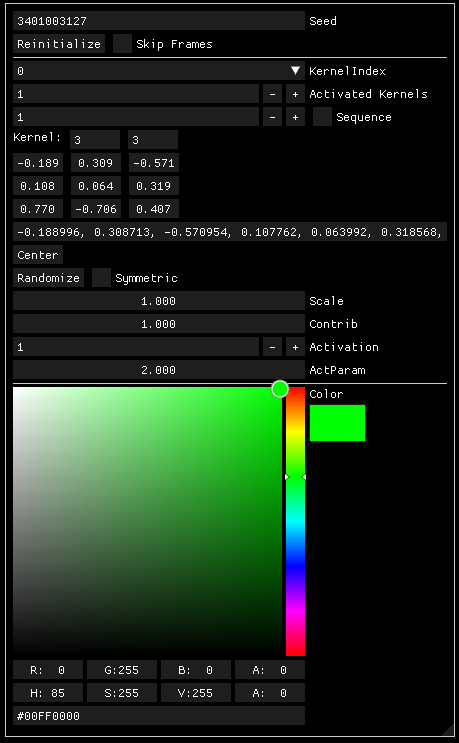
\includegraphics[width=2.0in]{imgs/gui.png}
}
\section{Results}
We begin with some a qualitative analysis of some examples of our method at various kernel depths, constraints, and kernel sizes.
The following patterns were generated with single-depth small kernels (3x3 or 4x4) paired with an activation function. The color channels used are purely visual, as the cellular automata do not interact across colors.
%1 layer non symmetric%
\adjustbox{center}{
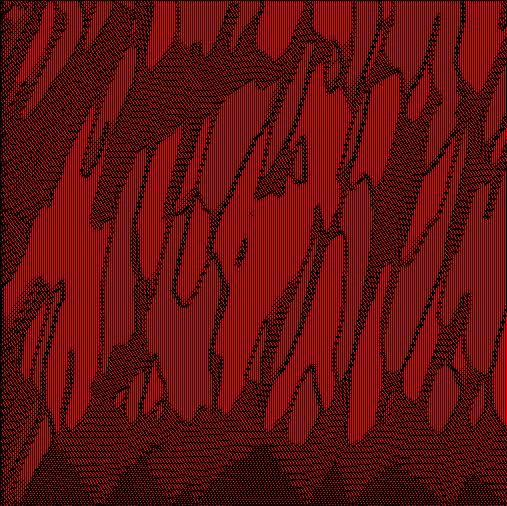
\includegraphics[width=2.0in]{imgs/red-cells.png}
}
\adjustbox{center}{
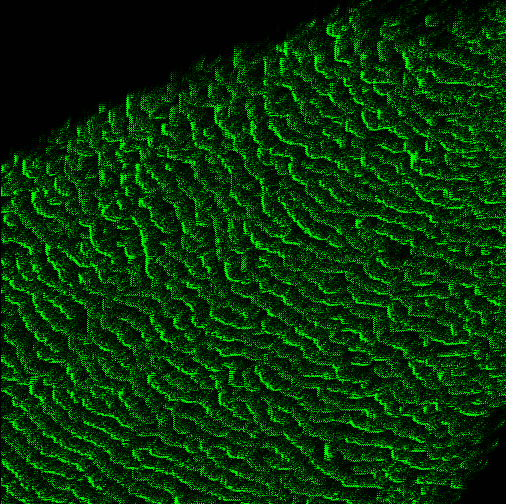
\includegraphics[width=2.0in]{imgs/growth-waves.png}
}
\adjustbox{center}{
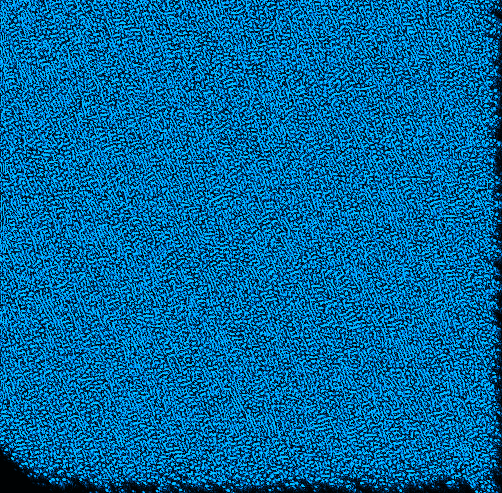
\includegraphics[width=2.0in]{imgs/swirly.png}
}
Even with this low model complexity, we do see rise of very interesting patterns and dynamic behavior. Although, we do start to see the anisotropic texture qualities previously described. We found that if motion is desired in the automata, we can control it by rotating the kernel weights by a desired angle, as well as modifying the CoM of the kernel to shift the motion strength and direction.

We naturally progress by continuing to use relatively small single kernels, but enforcing octant symmetry to produce symmetric motion and relatively anisotropic structured patterns. 
%1 layer symmetric%
\adjustbox{center}{
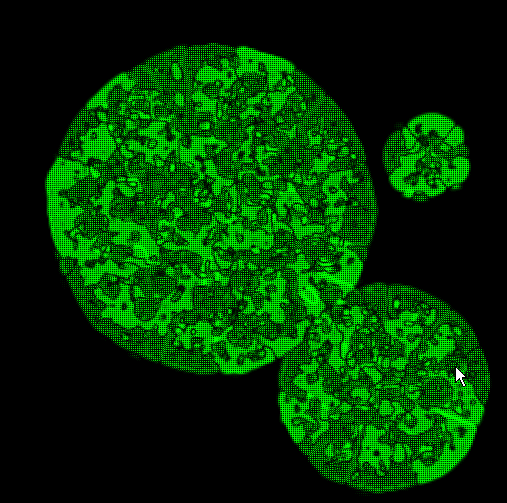
\includegraphics[width=2.0in]{imgs/bubbling-moss.png}
}
\adjustbox{center}{
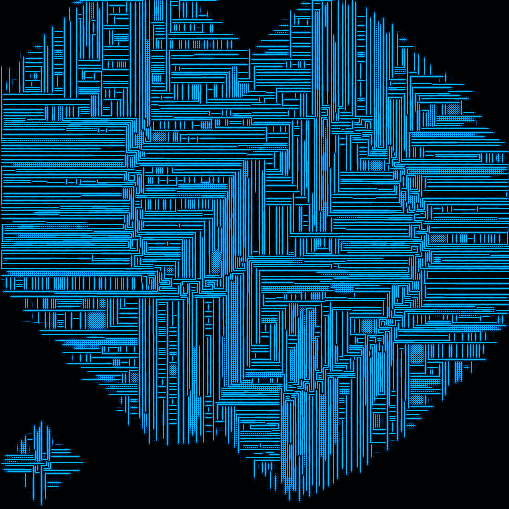
\includegraphics[width=2.0in]{imgs/blue-pipes.png}
}
\adjustbox{center}{
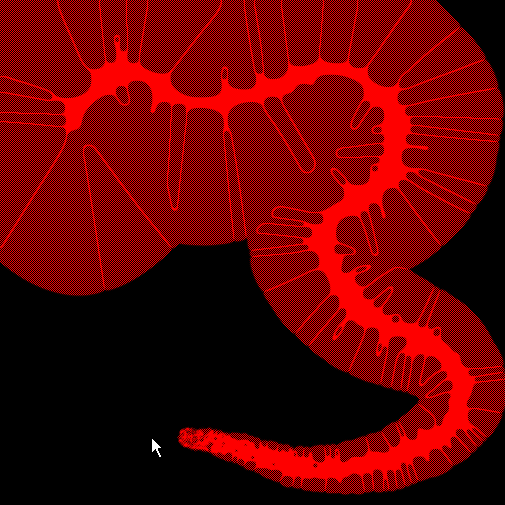
\includegraphics[width=2.0in]{imgs/slimy-snake.png}
}
\adjustbox{center}{
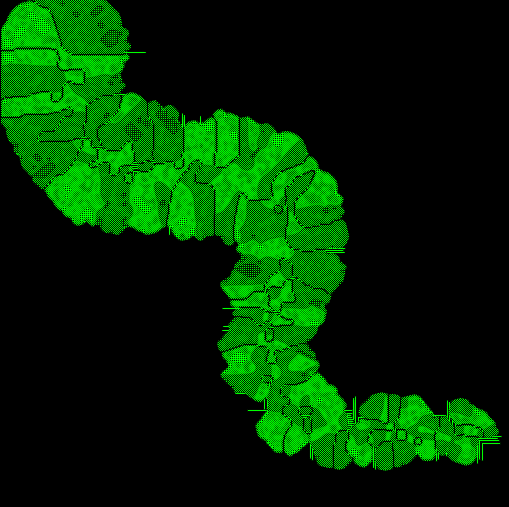
\includegraphics[width=2.0in]{imgs/slimy-pipes.png}
}
This symmetry enables much more predictable results when interacting with the domain as can be seen by the distinct trails and origins that arise due to user input.

Next we increase the model depth, adding up to 5 consecutive kernels each with an activation and custom scaling and contribution parameters.
%multi layered%
\adjustbox{center}{
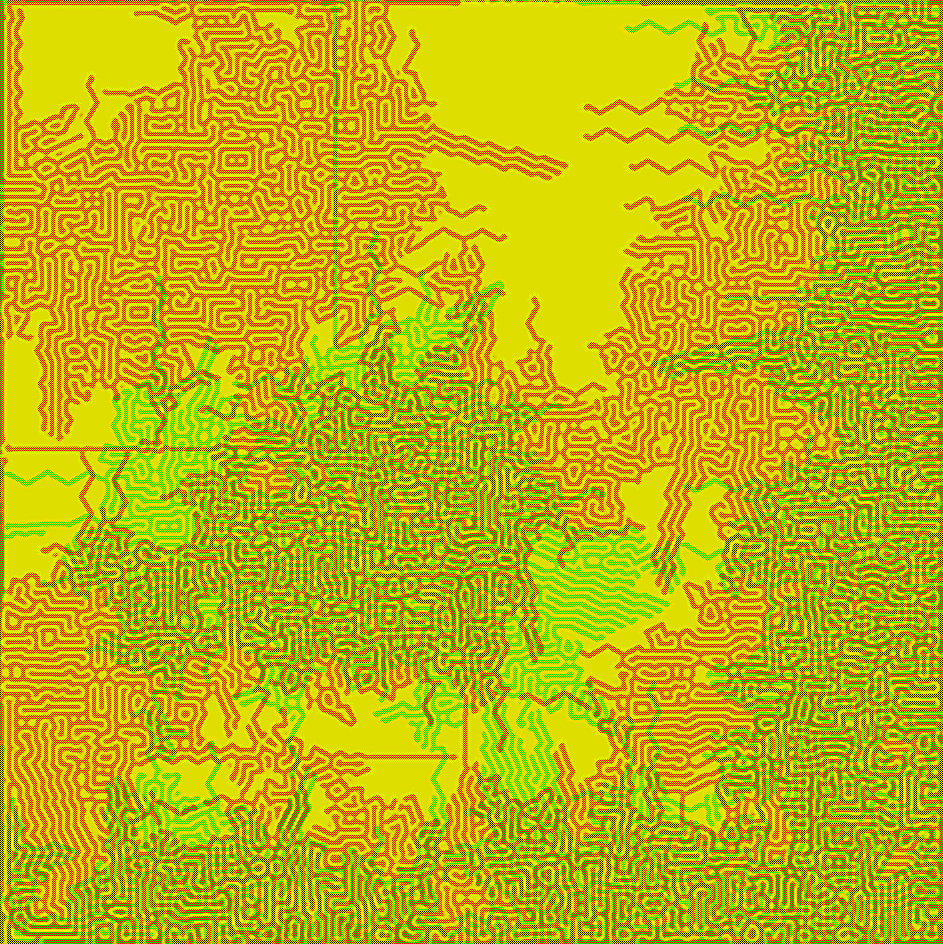
\includegraphics[width=2.0in]{imgs/redgreen-zigzag growth.png}
}
\adjustbox{center}{
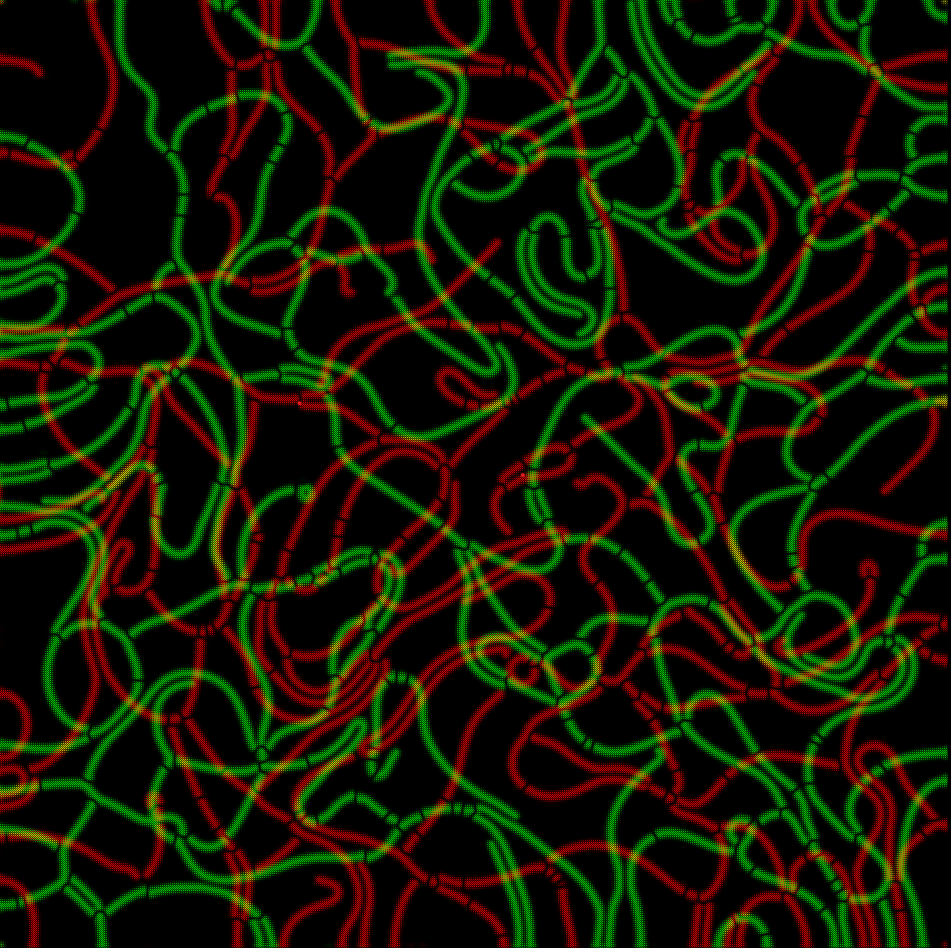
\includegraphics[width=2.0in]{imgs/aredgreen-spaghetti-worms.png}
}
\adjustbox{center}{
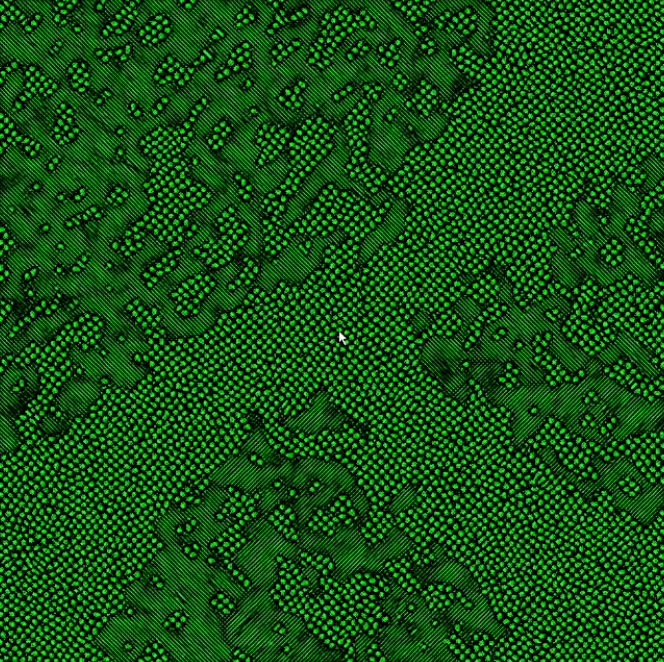
\includegraphics[width=2.0in]{imgs/bacteria.png}
}
We begin to see these aforementioned organic structures take shape both in their single-frame appearance and their evolution over time. In these examples, the worm-like structure evolves reminiscent of microscopic worms under a microscope, both searching their environment and avoiding competing organisms. We found many examples of creating bacteria-like patterns such as the last figure.

To understand the contribution of various kernel levels in the sequence, we show a few samples along with their intermediate outputs. One interesting, and sometimes frustrating, part of designing patterns in this manner are the sometimes hidden effects of kernels lower in the hierarchy that only begin to show their effects once layered deeper.
\adjustbox{center}{
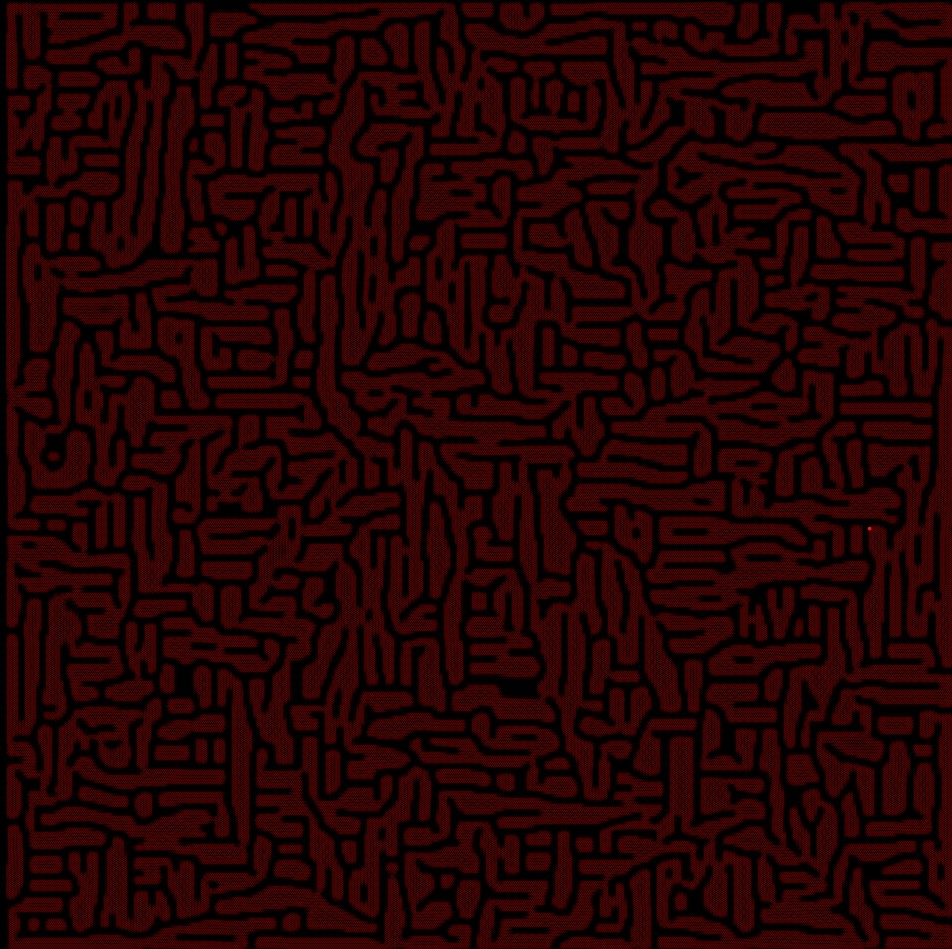
\includegraphics[width=1.0in]{imgs/pix-cells1.png}
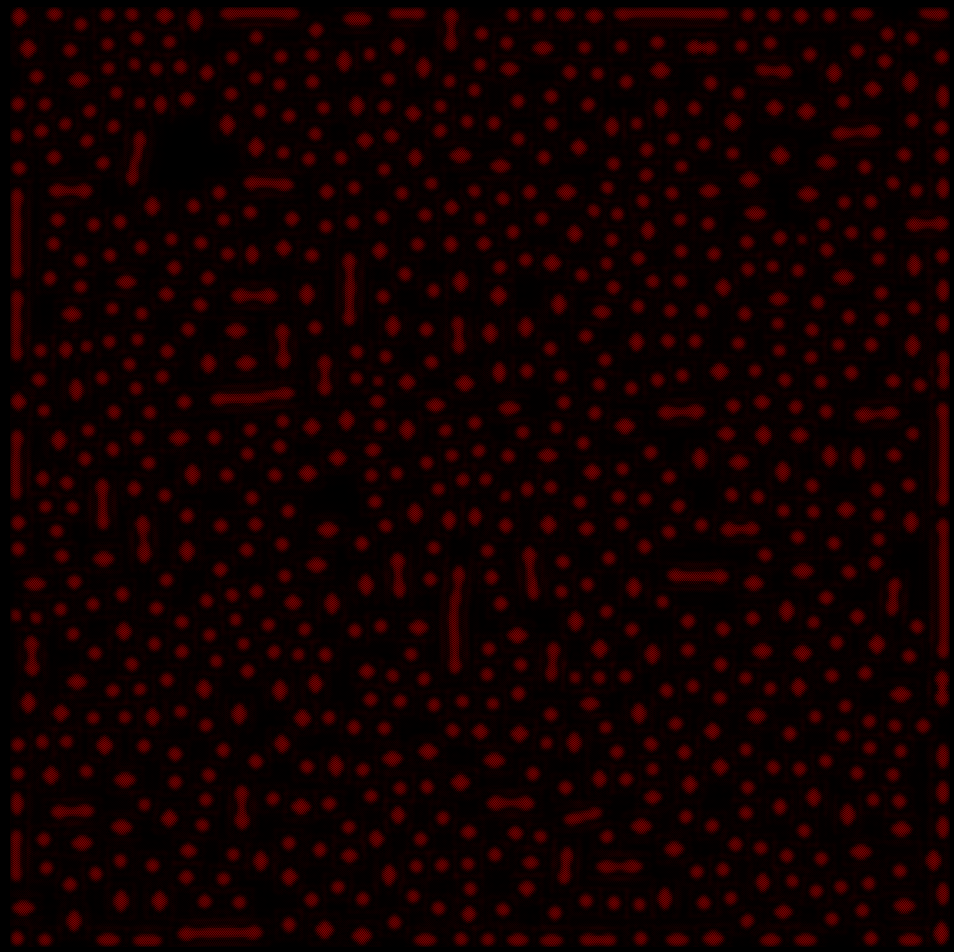
\includegraphics[width=1.0in]{imgs/pixcells2.png}
}
\adjustbox{center} {
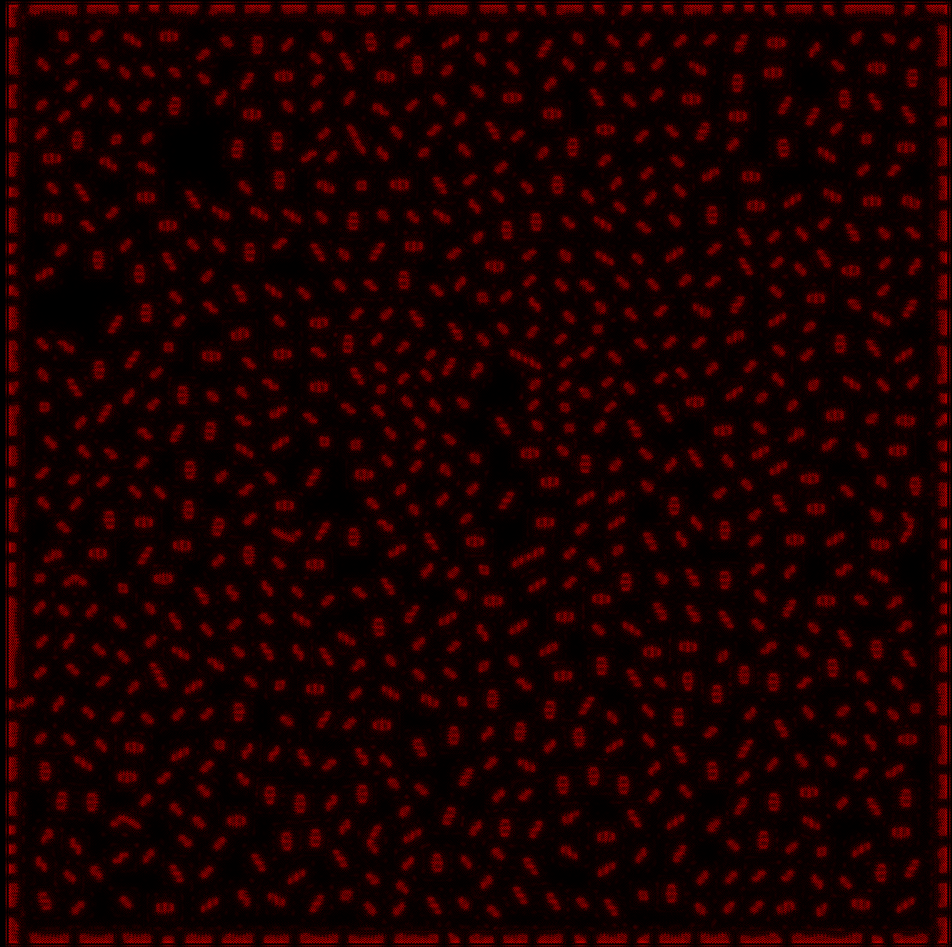
\includegraphics[width=1.0in]{imgs/pixcells4.png}
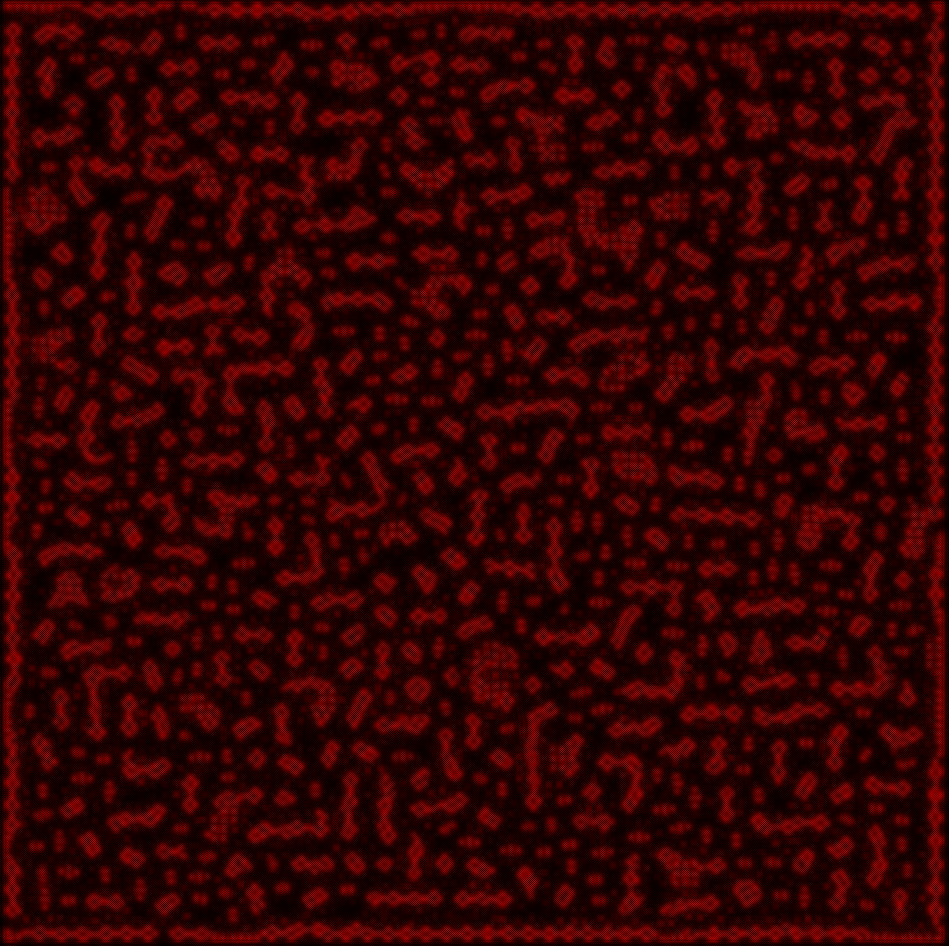
\includegraphics[width=1.0in]{imgs/pixcells5.png}
}
\adjustbox{center} {
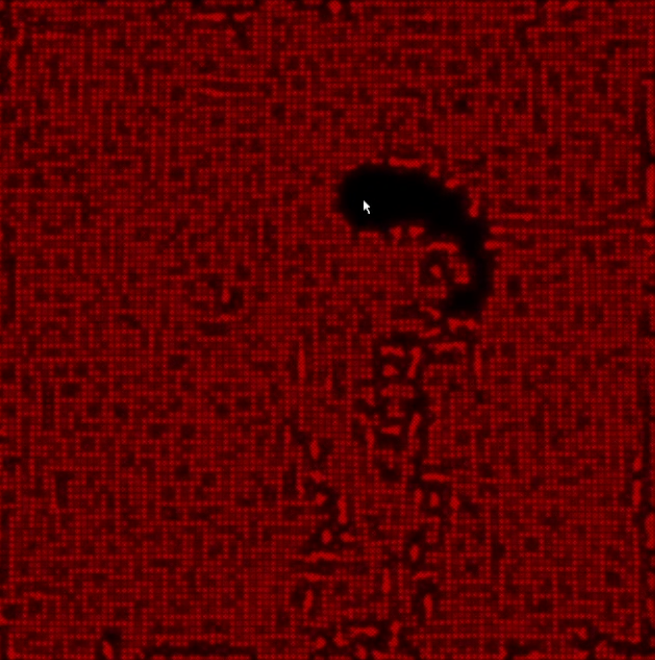
\includegraphics[width=2.0in]{imgs/pixelcells-interactive.png}
}
This 5-level kernel system shows the formation of worm-like structures on the later stages, but interstingly kernel 4 introduces an LCD pixel-like arrangement. In the final output, we demonstrate the self assembling properties of these systems as a user interactively clears a path through the domain. As previously mentioned, a good application of this would be to deform a floor texture based on player position in a scene.
\adjustbox{center}{
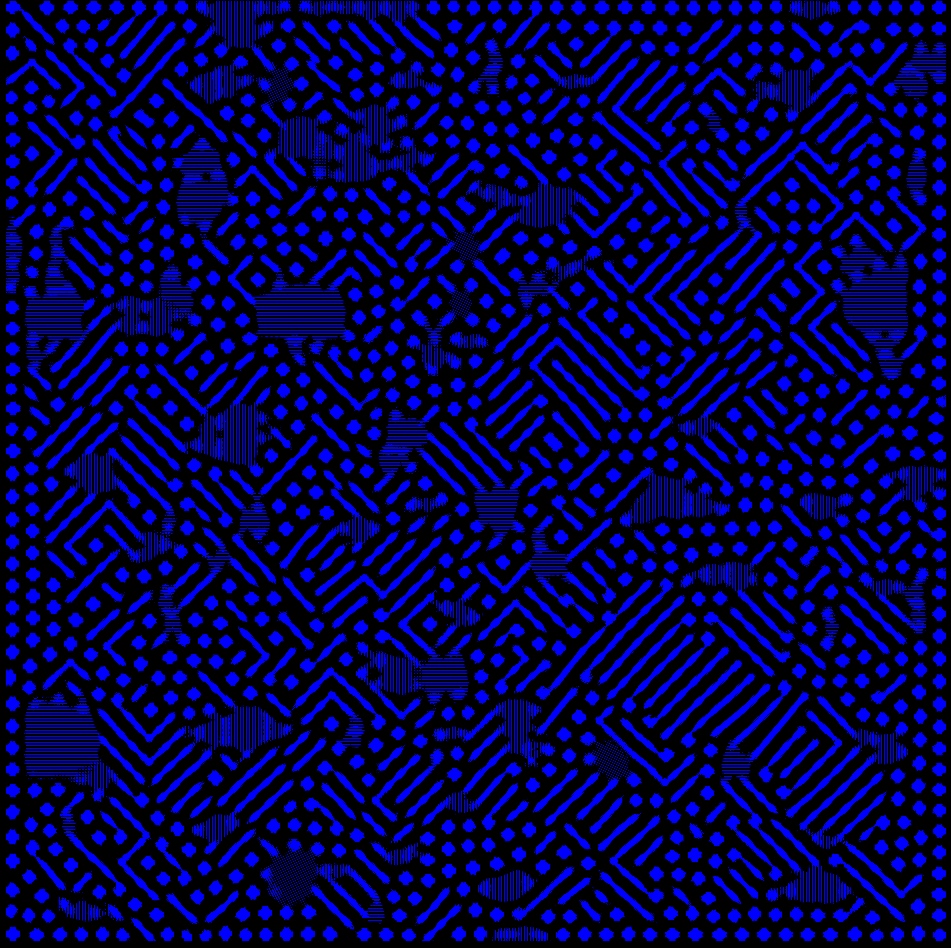
\includegraphics[width=1.0in]{imgs/comets1.png}
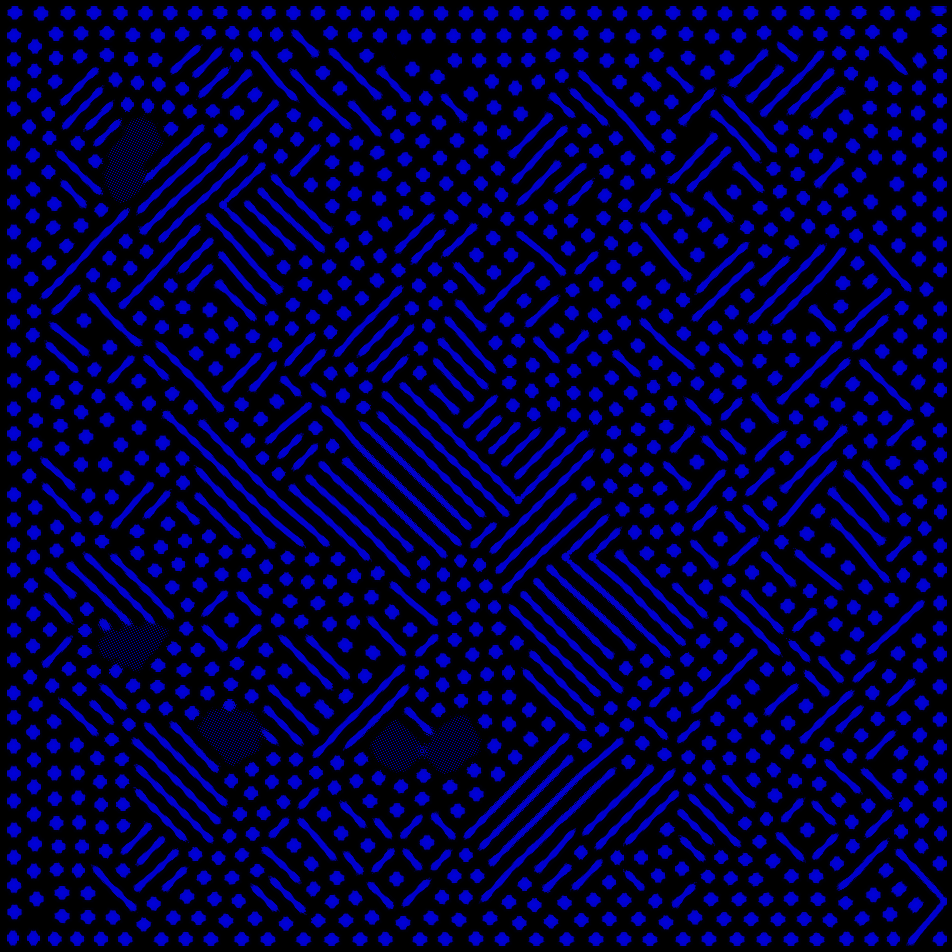
\includegraphics[width=1.0in]{imgs/comets2.png}
}
\adjustbox{center}{
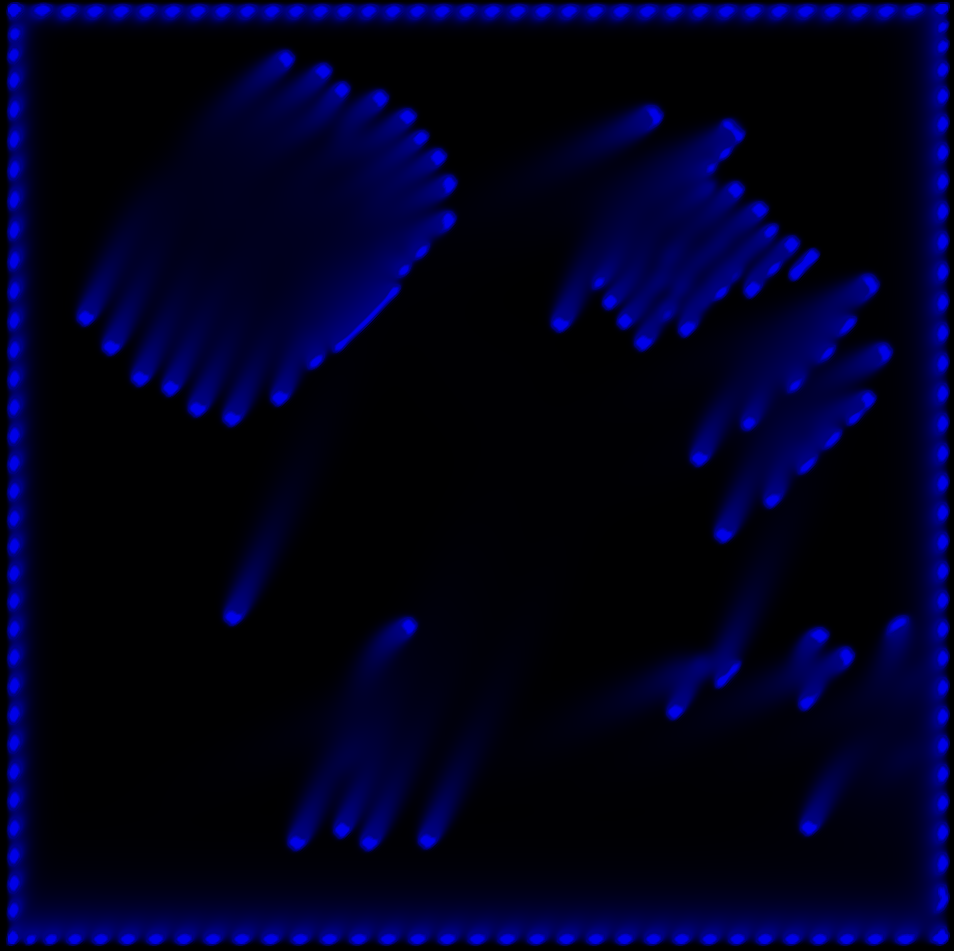
\includegraphics[width=2.0in]{imgs/comets3.png}
}
We were also able to generate dynamic effects, not just relatively stationary textures as previously shown. In the above example we see the two intermediary patterns form a relatively stable lattice without much variation between the levels. After we add the final kernel level however, we see comet-like effects emerge at user interaction points. Notably, although the second kernel level in isolation does not appear to modify the pattern behaviour very much, it is integral in the final motion and stability of the system. When omitted, the final output results in incoherent clearing of the image.
\adjustbox{center}{
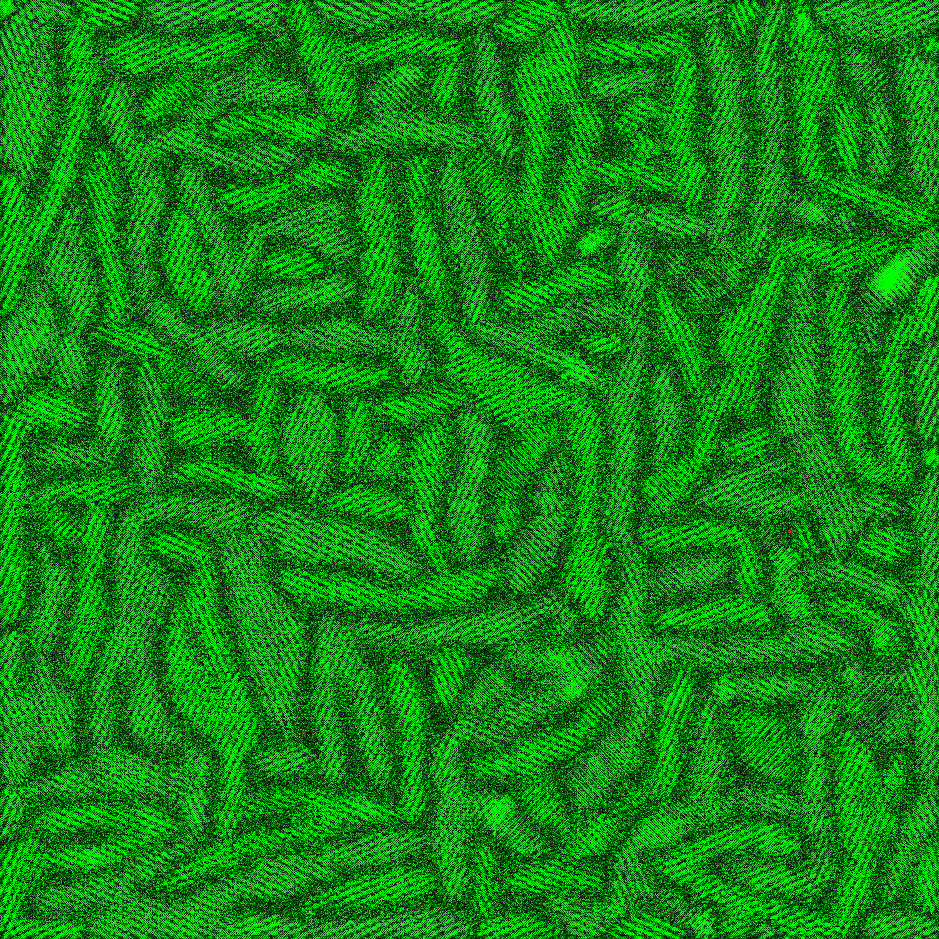
\includegraphics[width=1.0in]{imgs/mitosis1.png}
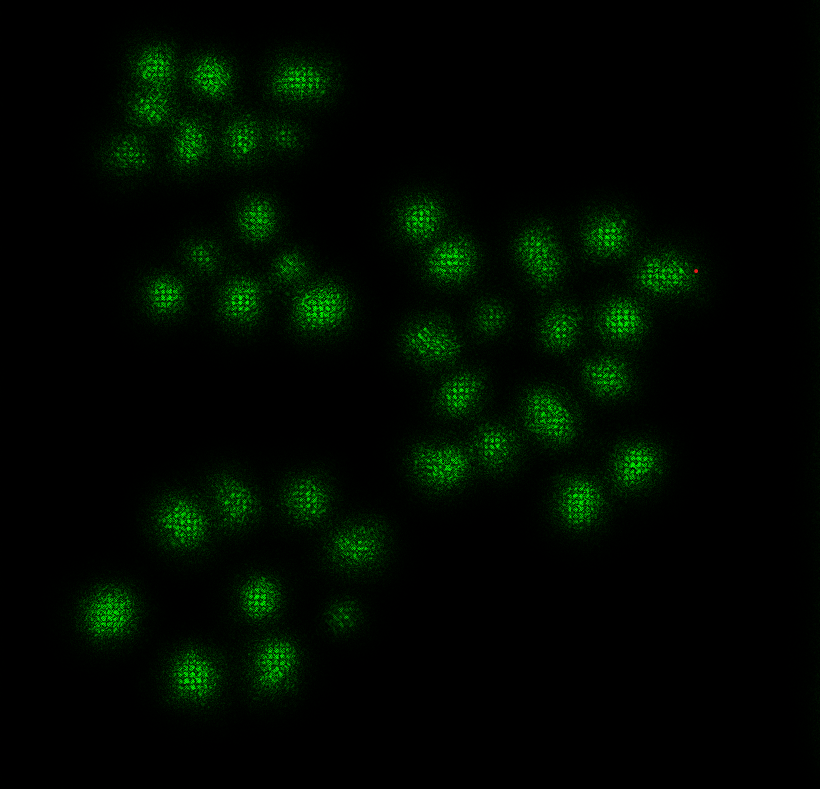
\includegraphics[width=1.0in]{imgs/mitosis2.png}
}
\adjustbox{center}{
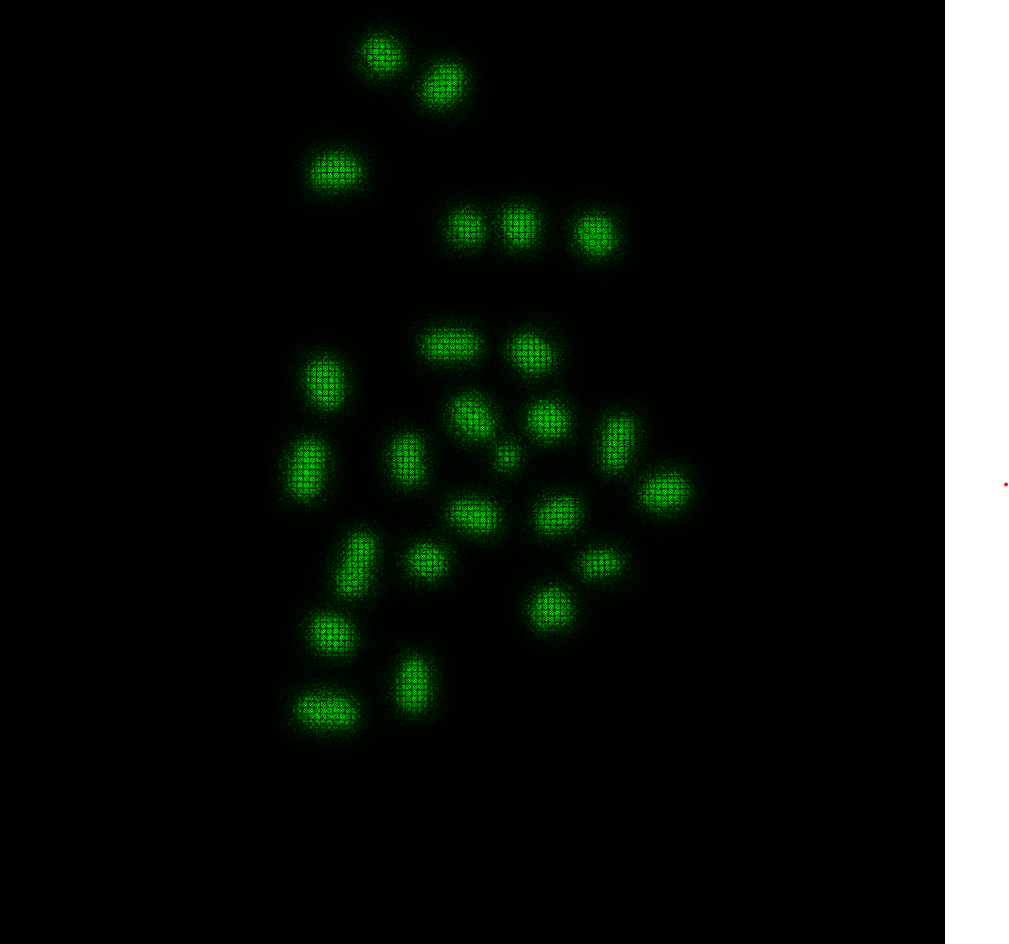
\includegraphics[width=2.0in]{imgs/mitosis3.png}
}
The final system demonstrates on of the most interesting emergent behaviours we found when exploring the feature space of our system. What begins with a worm-like noisy input quickly gives rise to cell structures that exhibit mitosis-like replication. This is an example where we apply a gaussian smoothing kernel as the final operator to reduce the noise within the cell structures and smooth their motion.

We give the following performance measurements as tested on an NVIDIA RTX 2070 Super graphics card, where the Vulkan graphics API was used to dispatch the compute shaders and manage resources. Our text images were simulated at a resolution of 960x960, and averaged over a simulation period of 60 seconds.

% Table 1: Single-Shot Kernel Times
\begin{table}[h]
\centering
\begin{tabular}{|c|c|}
\hline
\textbf{Kernel Size} & \textbf{Time (ms)} \\
\hline
3$\times$3 & 2.71 \\
7$\times$7 & 2.75 \\
13$\times$13 & 3.05 \\
17$\times$17 & 3.15 \\
21$\times$21 & 3.45 \\
\hline
\end{tabular}
\caption{Single-Shot Kernel Times}
\label{tab:single-shot}
\end{table}

% Table 2: 5-Level Kernel Times
\begin{table}[h]
\centering
\begin{tabular}{|c|c|}
\hline
\textbf{Kernel Size} & \textbf{Time (ms)} \\
\hline
3$\times$3 & 2.91 \\
7$\times$7 & 3.05 \\
13$\times$13 & 5.28 \\
17$\times$17 & 8.03 \\
21$\times$21 & 13.23 \\
\hline
\end{tabular}
\caption{5-Level Kernel Times}
\label{tab:five-level}
\end{table}

Although with deeper patterns it is rare to use multiple kernels of larger size, we do notice a significant performance dropoff in the multi-level worse case benchmark. With more optimized compute shaders, and leveraging shared group memory between thread workgroups we believe this performance can be reduced significantly. As it stands this strategy may be too costly to incorporate into AAA games, however smaller games that focus on this dynamic cellular automata as a core mechanic or art style direction will find the performance suitable, especially if simulation is not performed on every frame.

\section{Postmortem}
In general, we are pleasantly surprised by the project and the generated effects. It seems to enable effects that are not commonly used or seen in interactive media, and would be an interesting addition to game projects either as purely visual effects, or core game play mechanics. As modern GPUs and graphicsd APIs become more powerful, many game systems have begun to move to being implemented through compute shaders. We see our project as a natural progression of this new power, exploring how previously infeasible effects can be integrated in a game environment. We see the highly dynamic and interactive nature of our cellular automata framework an intersting and underexplored area of previously offline computer graphics techniques in games.
For a prototype system, our performance is promising. We are confident that with more optimizations such as shared workgroup memory pooling to reduce total number of texture reads in large kernels we can further reduce the simulation times and reach targets suitable for modern production games.
Like many cellular automata systems, our weak point remains in the authoring process. The reality is that although adding more layers to the model vastly increases the feature space of possible patterns, this also makes finding these patterns exponentially more challenging. The artist creation process for these effects is largely exploratory, and even with the tools and parameters we discussed, it can still be difficult to create a target effect when one is desired. Creating interesting systems requires a lot of tuning and balancing parameters by hand until a stable configuration is reached. We see improving this area as the natural next-step in making the adoption of these patterns in games. We believe there are still low hanging fruit extensions to narrow the feature search space, such as employing heuristics to automatically detect a range of parameters that do not ``explode'', creating a library of kernel primitives that can easily be combined to create desired effects, and employing a generational algorithm design approach where users can select between various slight mutations of the current system to get closer to a desired result.
\section{Conclusion}
We demonstrate to the best of our knowledge a novel application of multi-layered convolutional cellular automata for the use in dynamic textures and patterns in games. We describe our GPU pipeline architecture that allow the simulation of these patterns in highly interactive rates which would be required to integrate into a production system. Finally, we offer a reference implementation of a cellular automata authoring tool that allows user to create and save the various kernels levels and parameters they find. 

\pagebreak
\printbibliography
\end{document}
